\documentclass[11pt,a4paper]{article}

% Encoding and fonts
\usepackage[T1]{fontenc}
\usepackage[utf8]{inputenc}

% Math
\usepackage{amsmath}
\usepackage{amsfonts}
\usepackage{amssymb}

% Graphics and figures
\usepackage{graphicx}
\usepackage{booktabs}
\usepackage{float}

% Hyperlinks
\usepackage[colorlinks=true,linkcolor=blue,citecolor=blue,urlcolor=blue]{hyperref}

% Colors
\usepackage{xcolor}

% Bibliography
\usepackage[numbers]{natbib}

% Page geometry
\usepackage[margin=1in]{geometry}

% Tables
\usepackage{array}
\usepackage{caption}

% TikZ
\usepackage{tikz}
\usetikzlibrary{shapes,arrows,positioning,fit,backgrounds}


\title{\LARGE\bfseries From Self-Refine to Self-Evolve:\\A Unified Framework for AI Self-Evolution\\through Five Evolutionary Loops}

\author{
  Self Evolve Research Team\\[0.5em]
  \texttt{https://github.com/self-evolve}
}

\date{May 2026}

\begin{document}

\maketitle

\begin{abstract}
AI self-evolution---the ability of artificial systems to autonomously improve their own capabilities---is emerging as a unifying paradigm across multiple research communities. Rather than a single technique, we argue that self-evolution comprises five distinct but complementary loops: (1) the \textbf{Specification-to-Execution Loop}, which translates natural-language goals into runnable pipelines; (2) the \textbf{Search Loop}, which explores architectural, prompt, and code spaces; (3) the \textbf{Evaluator Loop}, which scores candidates through testing and benchmarking; (4) the \textbf{Reflection Loop}, which converts failures into verbal memory and feedback; and (5) the \textbf{Population Loop}, which maintains, selects, and recombines multiple candidates. We systematize 17+ core papers and 19+ open-source projects spanning inference-time self-improvement (Self-Refine, Reflexion, Self-Debug), training-time methods (SPIN, STaR, Constitutional AI, ReST-EM), evolutionary code discovery (AlphaEvolve, FunSearch, OpenEvolve), and self-evolving agent systems (ADAS, Darwin G\"{o}del Machine, Absolute Zero). Our contributions include: (i) a unified taxonomy that maps existing methods to the five loops; (ii) a detailed comparative analysis with benchmark data; (iii) a research landscape analysis covering academic lineages and open-source ecosystems; and (iv) an articulation of open problems and a roadmap toward production-grade self-evolving AI.
\end{abstract}

%-------------------------------------------------------------------
\section{Introduction}
\label{sec:introduction}

\subsection{From Static AI to Self-Evolving AI}

The dominant paradigm in AI development has been \emph{static deployment}: a model is trained, evaluated, and deployed without further modification. Improvements require human intervention---collecting new data, designing better architectures, or tuning hyperparameters. This cycle is slow, expensive, and fundamentally limited by human engineering bandwidth. Even the most capable models, once deployed, remain frozen: they cannot fix their own errors, adapt to distribution shifts, or discover new strategies for the tasks they face.

A convergent shift is occurring across multiple communities. Large language models (LLMs) can now critique and refine their own outputs~\citep{madaan2023selfrefine}. Evolutionary algorithms can use LLMs as mutation operators to discover new algorithms~\citep{novikov2025alphaevolve,romera2024funsearch}. Agent frameworks can modify their own architectures through code-level self-reference~\citep{hu2024adas,zhang2025dgm}. Reinforcement learning systems can generate their own training tasks and curricula~\citep{zhao2025absolute_zero}. These developments point toward a shared aspiration: AI systems that \emph{evolve themselves}.

This aspiration is not new---Schmidhuber's G\"{o}del Machine~\citep{schmidhuber2003godel} envisioned self-rewriting provably optimal code in 2003. What has changed is that the building blocks now exist. Modern LLMs possess sufficient code understanding to propose meaningful modifications, automated evaluators can verify candidate improvements in many domains, and computational infrastructure makes large-scale evolutionary search feasible. The convergence of these capabilities makes self-evolution a practical research program rather than a theoretical curiosity.

\subsection{What is AI Self-Evolution?}

We define \textbf{AI self-evolution} as any process by which an AI system autonomously improves one or more of its components---model weights, prompts, code, tool usage, or architectural design---through iterative cycles of generation, evaluation, and selection, without requiring human intervention in the improvement loop itself.

This definition is intentionally broad. It encompasses methods that operate at inference time (no weight changes, only context refinement), training time (weight updates driven by self-generated data), and architectural level (modifying the agent's own code). The common thread is the \emph{closure of the improvement loop}: the system evaluates its own outputs and uses those evaluations to drive subsequent improvements.

Critically, self-evolution does not require that the system operate with zero human involvement \emph{at any point}. Human involvement may set the initial goals, design the evaluation function, or provide safety constraints. The key criterion is that the \emph{improvement loop}---the cycle of generating candidates, evaluating them, and producing improved candidates---operates autonomously once initiated.

\subsection{Relation to Existing Concepts}

Self-evolution is related to, but distinct from, several established concepts:

\textbf{Continual learning} addresses the challenge of learning from non-stationary data streams without catastrophic forgetting. Self-evolution may employ continual learning techniques, but its focus is on the \emph{autonomous} improvement loop rather than the sequential data assumption. A continually learning system adapts to new data; a self-evolving system generates its own improvement trajectory.

\textbf{Online learning} updates models with each incoming data point. Self-evolution is broader: the ``data'' may be self-generated (as in STaR~\citep{zelikman2022star}) or derived from self-evaluation (as in Reflexion~\citep{shinn2023reflexion}). Online learning assumes an external data stream; self-evolution creates its own.

\textbf{Self-supervised learning} creates training signals from the structure of input data itself (e.g., masked language modeling). Self-evolution goes beyond pre-training objectives to include task-driven, performance-guided improvement loops that can operate across the entire lifecycle of a deployed system.

\textbf{AutoML} automates the design of machine learning pipelines. Self-evolution subsumes AutoML as a special case---where the system being optimized is itself an ML pipeline---but extends to agent architectures, code, and multi-step workflows that go far beyond traditional ML pipeline design.

\textbf{Meta-learning} learns to learn across tasks. Self-evolution may use meta-learning as a mechanism, but it also includes non-parametric improvement (e.g., prompt evolution, code modification) that does not involve gradient-based meta-learning.

\subsection{Contributions}

This paper makes the following contributions:
\begin{enumerate}
\item A \textbf{unified taxonomy} of five evolution loops that categorizes existing self-improvement and evolutionary methods into a coherent framework, enabling systematic comparison and identifying gaps in current approaches.
\item A \textbf{systematic analysis} of 17+ core papers and 19+ open-source projects, with detailed method descriptions, key formulas, benchmark data, and cross-method comparisons grounded in actual experimental results.
\item A \textbf{cross-domain perspective} that bridges AutoML, neural architecture search (NAS), LLM self-improvement, evolutionary computation, and agent research---fields that have been developing in parallel but share fundamental mechanisms.
\item A \textbf{research landscape analysis} covering academic lineages, institutional networks, and the open-source ecosystem, revealing the concentration of innovation in a small number of highly connected research groups.
\item An articulation of \textbf{open problems} and a concrete roadmap toward production-grade self-evolving AI, including the Self-Evolve vision of an evolution layer above existing agent frameworks.
\end{enumerate}

\subsection{Paper Structure}

Section~\ref{sec:taxonomy} introduces the five-loop taxonomy with detailed descriptions and a comparative table. Section~\ref{sec:self-improvement} covers self-improvement methods at inference and training time, including key formulas and benchmark data. Section~\ref{sec:evolutionary-code} examines evolutionary code and algorithm discovery, from OPRO to AlphaEvolve. Section~\ref{sec:agent-evolution} surveys self-evolving agent systems, including architecture, workflow, and memory evolution. Section~\ref{sec:frameworks} analyzes agent frameworks and identifies capability gaps. Section~\ref{sec:automl-nas} explores the intersection of AutoML, NAS, and LLMs. Section~\ref{sec:landscape} maps the research community. Section~\ref{sec:future} identifies open problems and future directions. Section~\ref{sec:conclusion} concludes with a summary and the Self-Evolve vision.

\subsection{Related Surveys}

Several concurrent surveys cover overlapping territory. \citet{survey2024selfevolution} provides a broad taxonomy of self-evolving agents across model, context, tool, and architecture dimensions. The present work differs in its focus on the \emph{five evolution loops} as a unifying mechanism and its deeper technical analysis of specific methods with benchmark data. \citet{snell2024rise} studies test-time compute scaling, which relates to our inference-time self-improvement loop but does not address training-time or population-level evolution. We complement these works by providing a mechanism-level decomposition of how self-evolution operates across different timescales and system components.

%-------------------------------------------------------------------
\section{Taxonomy: Five Evolution Loops}
\label{sec:taxonomy}

We propose that AI self-evolution can be decomposed into five distinct but complementary loops, each capturing a fundamental mechanism by which systems improve themselves. A single method may engage multiple loops simultaneously; the most powerful systems combine all five. This decomposition is inspired by the observation that biological evolution itself operates through multiple interlocking mechanisms (variation, selection, inheritance, drift, speciation), and that artificial self-evolution similarly requires multiple interacting processes.

\begin{figure}[t]
\centering
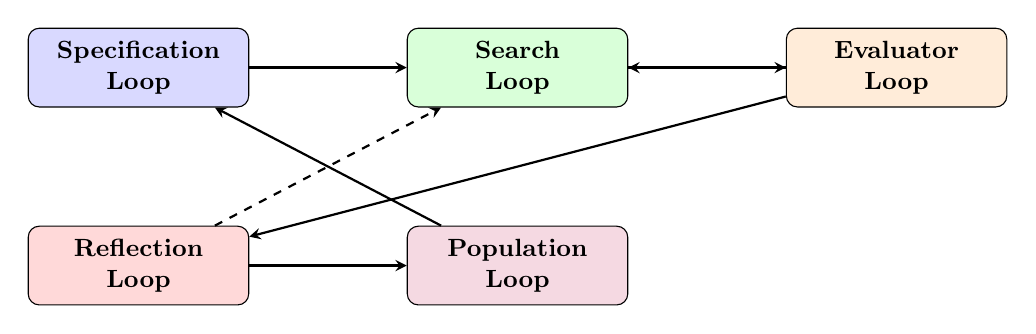
\begin{tikzpicture}[
  loop/.style={rectangle, draw, rounded corners, minimum width=2.8cm, minimum height=1cm, align=center, font=\small\bfseries},
  arrow/.style={->, thick, >=stealth},
  node distance=1.5cm and 2cm
]
  \node[loop, fill=blue!15] (spec) {Specification\\Loop};
  \node[loop, fill=green!15, right=of spec] (search) {Search\\Loop};
  \node[loop, fill=orange!15, right=of search] (eval) {Evaluator\\Loop};
  \node[loop, fill=red!15, below=of spec] (reflect) {Reflection\\Loop};
  \node[loop, fill=purple!15, right=of reflect] (pop) {Population\\Loop};

  \draw[arrow] (spec) -- (search);
  \draw[arrow] (search) -- (eval);
  \draw[arrow] (eval) -- (reflect);
  \draw[arrow] (reflect) -- (pop);
  \draw[arrow] (pop) -- (spec);
  \draw[arrow, dashed] (eval) -- (search);
  \draw[arrow, dashed] (reflect) -- (search);
\end{tikzpicture}
\caption{The five evolution loops and their interconnections. Solid arrows indicate the primary flow from specification through search, evaluation, reflection, and population management back to specification. Dashed arrows indicate feedback paths: evaluation scores guide search, and reflections inform future search strategies.}
\label{fig:five-loops}
\end{figure}

\subsection{Specification-to-Execution Loop}

The specification loop converts high-level natural-language goals into executable ML pipelines or agent workflows. The system takes a user's intent expressed in natural language and produces a fully functional system---selecting models, composing tools, and configuring parameters---without manual engineering.

\textbf{Representative systems.} AutoML-GPT~\citep{automlgpt2023} uses GPT-4 to interpret user requirements and select from a fixed toolbox of ML operations including data preprocessing, feature engineering, model selection, and hyperparameter optimization. AutoML-Agent~\citep{automlagent2024} extends this with multi-agent collaboration, where specialized agents handle data processing, model selection, and evaluation separately, achieving better pipeline quality through division of labor. These systems demonstrate that the gap between specification and execution can be bridged by LLMs that understand both the problem domain and the available technical components.

\textbf{Mechanism.} The specification loop operates through a mapping $f: \text{NL goals} \to \text{executable pipeline}$. The LLM decomposes the natural language specification into sub-tasks, selects appropriate tools or models for each sub-task, and composes them into a pipeline. Evaluation of the pipeline's output provides feedback for refinement, though current systems typically require human approval rather than fully autonomous iteration.

\textbf{Limitations.} Current systems are constrained by their fixed tool libraries---they can compose existing tools but cannot invent new ones. The specification loop becomes truly self-evolving only when the system can \emph{invent new tools} rather than merely composing existing ones---a capability that requires engaging the search and population loops.

\subsection{Search Loop}

The search loop explores a space of candidates---architectures, prompts, code, agent designs, or hyperparameters---to find high-performing configurations. Unlike gradient-based optimization, the search loop operates in discrete, non-differentiable spaces and relies on LLMs as proposal generators.

\textbf{Representative methods.} OPRO~\citep{yang2023opro} treats optimization as a natural-language process: the LLM receives a history of (solution, score) pairs and proposes new candidates, demonstrating that LLMs can serve as general-purpose optimizers without domain-specific heuristics. EvoPrompting~\citep{chen2024evoprompting} applies evolutionary search to neural architecture discovery, treating network descriptions as evolvable code that can be mutated and recombined. ADAS~\citep{hu2024adas} searches the space of all possible Python programs that implement agent architectures---a Turing-complete search space that encompasses any computable agent design.

\textbf{Key insight.} The search loop's power derives from the LLM's ability to perform \emph{structured variation}: it can propose mutations that are semantically meaningful (e.g., ``add a verification step before the final output'' rather than random token substitutions). This makes LLM-driven search qualitatively different from traditional evolutionary algorithms that rely on random perturbation. The LLM brings domain knowledge, common-sense reasoning, and pattern recognition to the variation operation, producing candidates that are far more likely to be improvements.

\textbf{Search space considerations.} The choice of search space determines what is evolvable. Prompt spaces are easy to search but limited in expressiveness. Architecture spaces (code-level descriptions) are Turing-complete but require more capable LLMs to propose meaningful modifications. The most productive search spaces balance expressiveness with searchability---they are large enough to contain novel solutions but structured enough for the LLM to navigate effectively.

\subsection{Evaluator Loop}

The evaluator loop provides the fitness signal that drives all other loops. Without reliable evaluation, self-evolution is blind: the system cannot distinguish improvements from regressions. The evaluator loop is arguably the most critical and most bottlenecked component of self-evolution.

\textbf{Representative methods.} FunSearch~\citep{romera2024funsearch} pairs an LLM with an automated evaluator that verifies mathematical correctness, enabling the discovery of new algorithms that no human had previously found. Self-Debug~\citep{chen2024selfdebug} uses execution feedback (error messages, stack traces, test outcomes) as the evaluation signal for iterative code repair, grounding the improvement loop in objective program behavior. CodeEvolve~\citep{wang2024codeevolve} uses benchmark performance on coding tasks as its evaluation function, measuring both functional correctness and computational efficiency.

\textbf{Types of evaluation.} Evaluators range along a spectrum from fully automated to fully human:
\begin{itemize}
\item \textbf{Automated verifiers}: Unit tests, mathematical proofs, code execution. Fast, objective, but limited to verifiable domains.
\item \textbf{LLM-as-judge}: Using a separate LLM to evaluate outputs. Scalable but introduces model-dependent biases.
\item \textbf{Human evaluation}: The gold standard for quality but expensive and slow, creating a bottleneck for iterative improvement.
\item \textbf{Hybrid approaches}: Combining automated metrics with periodic human validation to calibrate the automated evaluator.
\end{itemize}

\textbf{Critical challenge.} The evaluator loop is the bottleneck of self-evolution. In domains where automated evaluation is available (mathematics, programming, games), progress has been rapid. In domains requiring human judgment (creative writing, strategic planning, ethical reasoning), the evaluator loop remains the primary obstacle. The risk is that systems over-optimize for easily measurable benchmarks at the expense of genuine capability---a phenomenon already observed in code generation benchmarks where high HumanEval scores do not reliably predict real-world coding ability.

\subsection{Reflection Loop}

The reflection loop converts evaluation outcomes---particularly failures---into structured feedback that guides future improvement. Unlike raw evaluation scores (which are scalar signals), reflective feedback is \emph{explanatory}: it identifies \emph{why} a candidate failed and \emph{what} to change. This explanatory quality is what makes reflection a distinct loop rather than a subset of evaluation.

\textbf{Representative methods.} Self-Refine~\citep{madaan2023selfrefine} uses a single LLM to generate, critique, and refine its own output in an iterative loop, achieving approximately 20\% improvement across seven tasks without any training. Reflexion~\citep{shinn2023reflexion} stores linguistic feedback in a persistent memory buffer that grows across episodes, achieving 91\% pass@1 on HumanEval compared to GPT-4's 80\%. STaR~\citep{zelikman2022star} employs ``rationalization''---generating post-hoc reasoning chains for incorrect answers---to bootstrap reasoning capabilities, enabling a 540M-parameter model to match the performance of a 175B model.

\textbf{Key insight.} The reflection loop operates as a form of ``verbal gradient descent'': instead of computing numerical gradients through a differentiable loss function, the system generates natural-language explanations of errors and uses these to steer subsequent generations. The linguistic feedback serves as a directional signal that guides the search toward better regions of the solution space. This is both a strength (works in non-differentiable domains where gradient-based methods cannot operate) and a limitation (quality depends on the LLM's ability to accurately diagnose its own errors, which degrades for complex or subtle failures).

\textbf{Memory persistence.} A key design choice is whether reflections persist across episodes. Self-Refine discards feedback after each refinement cycle, limiting its learning to the current task. Reflexion maintains a growing memory buffer, enabling cross-episode learning where feedback from failed attempts on one problem helps solve related problems. The trade-off is between context window consumption (larger memory buffers consume more tokens) and learning transfer (persistent memory enables broader knowledge accumulation).

\subsection{Population Loop}

The population loop maintains a diverse collection of candidates, enabling selection, recombination, and specialization beyond what a single trajectory can achieve. It is the mechanism that transforms sequential improvement into open-ended exploration.

\textbf{Representative methods.} AlphaEvolve~\citep{novikov2025alphaevolve} uses MAP-Elites quality-diversity search~\citep{mouret2015mapelites} to maintain an archive of high-performing solutions mapped across behavioral dimensions, discovering the first improvement over Strassen's matrix multiplication algorithm in 56 years. LLaMEA~\citep{lanzi2024llamea} maintains a population of algorithm candidates and uses the LLM to propose mutations, winning the GECCO Silver Humies award for human-competitive results. The Darwin G\"{o}del Machine~\citep{zhang2025dgm} maintains an open-ended archive of agent implementations, improving SWE-bench performance from 20.0\% to 50.0\% through cumulative architectural discoveries.

\textbf{Key insight.} Population-level evolution enables \emph{stepping stones}: intermediate solutions that are not optimal for the target task but provide the genetic material for future breakthroughs. This is why AlphaEvolve could surpass human mathematical intuition---it explored paths that no single optimization trajectory would have taken, accumulating partial solutions that eventually combined into a novel algorithm. MAP-Elites ensures that the population maintains diversity across behavioral dimensions, preventing premature convergence to local optima.

\textbf{Recombination vs.\ mutation.} Population methods can produce new candidates through two mechanisms: \emph{mutation} (modifying a single parent) and \emph{recombination} (combining elements from multiple parents). LLMs are particularly well-suited for recombination because they can identify and integrate functional components from different candidates---for example, combining a promising initialization strategy from one agent with an effective error-handling mechanism from another.

\subsection{Cross-Loop Comparison}

Table~\ref{tab:loop-comparison} summarizes the five loops along key dimensions. The key observation is that the loops are complementary: each addresses a different aspect of the self-evolution process, and the most capable systems engage multiple loops simultaneously.

\begin{table}[t]
\centering
\caption{Comparison of the five evolution loops. Each loop captures a distinct mechanism for self-improvement.}
\label{tab:loop-comparison}
\small
\begin{tabular}{@{}p{2cm}p{2.5cm}p{2.5cm}p{2cm}p{2.5cm}@{}}
\toprule
\textbf{Loop} & \textbf{Input} & \textbf{Output} & \textbf{State} & \textbf{Representative} \\
\midrule
Specification & Natural language goals & Executable pipeline & None & AutoML-GPT \\
Search & Candidate space & New candidates & Search history & OPRO, ADAS \\
Evaluator & Candidate solution & Fitness score & None & FunSearch, Self-Debug \\
Reflection & Failure outcome & Verbal feedback & Memory buffer & Reflexion, Self-Refine \\
Population & Multiple candidates & Selected/recombined & Archive & AlphaEvolve, DGM \\
\bottomrule
\end{tabular}
\end{table}

%-------------------------------------------------------------------
\section{Self-Improvement Methods}
\label{sec:self-improvement}

This section analyzes methods that enable AI systems to improve their own outputs or weights through iterative self-feedback, without external human annotation in the improvement loop. We organize these methods into inference-time approaches (which modify outputs without changing weights) and training-time approaches (which permanently update model parameters), then analyze the trade-offs between these paradigms.

\subsection{Inference-Time Self-Improvement}

Inference-time methods improve outputs without modifying model weights. The model generates, evaluates, and refines its own responses at test time, using additional compute to trade for better performance. This is closely related to the test-time compute scaling paradigm~\citep{snell2024rise}, where additional inference passes are used to improve output quality.

\subsubsection{Self-Refine}

Self-Refine~\citep{madaan2023selfrefine} is perhaps the simplest self-improvement mechanism: a single LLM iteratively generates, critiques, and refines its own output. The three-step loop operates as follows:

\begin{enumerate}
\item \textbf{Generate}: The model produces an initial output $y_0 = \text{LLM}(x, \text{instruction})$.
\item \textbf{Critique}: The model analyzes $y_0$ against a task-specific rubric, producing feedback $\text{fb}_0 = \text{LLM}(y_0, \text{rubric})$.
\item \textbf{Refine}: The model produces an improved output $y_1 = \text{LLM}(y_0, \text{fb}_0, \text{instruction})$.
\end{enumerate}

This loop repeats until the critique indicates no further improvements are needed or a maximum iteration count is reached. Self-Refine achieves approximately 20\% improvement across seven diverse tasks, including code optimization (+28\%), sentiment reversal (+12 percentage points), math reasoning (+11pp), dialogue response quality (+16pp win rate), and constrained generation (+13pp compliance). Its key strength is simplicity---it requires no training, no external feedback, and no architecture changes, making it applicable to any capable LLM out of the box.

Its key limitation is convergence to local optima: the model's self-critique may fail to identify fundamental flaws in its own reasoning, particularly for complex tasks where the error is not locally apparent. The model can only refine within the scope of its own understanding---if the initial generation starts from a fundamentally wrong approach, iterative refinement may polish the wrong solution rather than discovering a better one.

\subsubsection{Reflexion}

Reflexion~\citep{shinn2023reflexion} extends the self-improvement paradigm by introducing persistent verbal memory. Rather than discarding feedback after each refinement, Reflexion stores linguistic self-reflections in a growing memory buffer that persists across episodes:

\begin{enumerate}
\item The \textbf{Actor} generates an action $a_e = M_a(\text{task}, M_{1:e-1})$ given the task and accumulated memory.
\item The \textbf{Evaluator} scores the action: $r_e = M_e(a_e, \text{task})$.
\item If $r_e$ indicates failure, the \textbf{Self-Reflection} module generates feedback $f_e = M_r(a_e, r_e, \text{task})$ describing what went wrong and what to do differently.
\item The memory is updated: $M_e = M_{e-1} \cup \{f_e\}$.
\end{enumerate}

This mechanism acts as ``verbal gradient descent''---natural language feedback replaces numerical gradients. Reflexion achieves 91\% pass@1 on HumanEval (surpassing GPT-4's 80\%), 97\% success on AlfWorld interactive environments (vs.\ 75\% baseline), and improvements on WebShop reward metrics. The persistent memory buffer enables cross-episode learning: feedback from failed attempts on one problem helps solve related problems.

The three-model architecture (Actor, Evaluator, Self-Reflection) is a design choice that separates concerns: the Actor focuses on generation, the Evaluator provides objective assessment, and the Self-Reflection module produces actionable feedback. This separation allows each component to be independently optimized or replaced.

\subsubsection{Self-Debug}

Self-Debug~\citep{chen2024selfdebug} specializes the reflection loop for code generation. Given generated code that fails unit tests, the model receives execution feedback (error messages, stack traces, test outcomes) and iteratively repairs the code. The key innovation is using \emph{execution traces} as the feedback signal rather than self-generated critiques. This grounds the improvement loop in objective program behavior rather than the model's potentially flawed self-assessment. Self-Debug demonstrates that even when a model cannot accurately critique its own logic, execution feedback provides a reliable signal for iterative improvement.

\subsection{Training-Time Self-Improvement}

Training-time methods modify model weights using self-generated training signals, enabling permanent capability improvements that persist across inference sessions. These methods go beyond inference-time refinement by creating lasting changes to the model's parameters.

\subsubsection{SPIN: Self-Play Fine-Tuning}

SPIN~\citep{spin2024} models LLM fine-tuning as a two-player zero-sum game. The current model $\theta_{t+1}$ (the ``main player'') learns to distinguish its own previous outputs from human-written responses. The previous iteration's model $\theta_t$ (the ``opponent'') generates the synthetic data. The training objective is:

\begin{equation}
L_{\text{SPIN}}(\theta) = \mathbb{E}_{x \sim \mathcal{D}} \left[ \mathbb{E}_{y \sim p_{\text{data}}} \left[ \log \sigma\left( \lambda \left( h_\theta(x, y) - h_\theta(x, \tilde{y}) \right) \right) \right] \right]
\end{equation}

\noindent where $h_\theta(x,y) = \log p_\theta(y|x)$, $\tilde{y} \sim p_{\theta_t}(\cdot|x)$ is the opponent's generation, and $\sigma(\cdot)$ is the logistic function. A key theoretical result is the convergence theorem: the global optimum $\theta^*$ satisfies $p_{\theta^*} = p_{\text{data}}$, meaning the model distribution exactly matches the human data distribution.

SPIN converges within approximately 3 iterations---the opponent can no longer generate responses that are distinguishable from human data. Remarkably, SPIN outperforms DPO trained with GPT-4 preference data on the HuggingFace Open LLM Leaderboard, while using only the original SFT dataset. This demonstrates that self-play can substitute for expensive human annotation: the model learns to improve by competing against its own past versions rather than by learning from external preferences.

\subsubsection{STaR: Self-Taught Reasoner}

STaR~\citep{zelikman2022star} bootstraps reasoning capability through an iterative generate-filter-finetune loop with a crucial ``rationalization'' mechanism:

\begin{enumerate}
\item \textbf{Generate}: For each problem $x_i$, the model produces a reasoning chain $r_i$ and answer $\hat{y}_i$.
\item \textbf{Filter}: Retain only $(x_i, r_i)$ pairs where $\hat{y}_i = y_i$ (correct answer).
\item \textbf{Rationalize}: For incorrect answers, provide the correct $y_i$ as a hint and regenerate the reasoning chain $r_i' = \arg\max_r p_\theta(r | x_i, y_i, F)$.
\item \textbf{Finetune}: Update the model on all successful reasoning chains, including rationalized ones.
\end{enumerate}

The rationalization step is STaR's key innovation. By ``working backward'' from correct answers, the model generates training data for problems it initially failed. This is analogous to a student who, upon seeing the correct answer to a problem they got wrong, constructs an explanation for why that answer is correct. The finetuning objective is:

\begin{equation}
\mathcal{L} = -\sum_{(x,r) \in D_{\text{correct}}} \log p_\theta(r | x, F)
\end{equation}

\noindent STaR enables a 540M-parameter model to achieve 72.5\% on CommonsenseQA---matching a 175B model that is 30$\times$ larger. This demonstrates that self-generated reasoning data can substitute for scale, and that the generate-filter-rationalize-finetune cycle is a powerful paradigm for bootstrapping capabilities from limited initial competence.

\subsubsection{Constitutional AI}

Constitutional AI~\citep{bai2022constitutional} introduces a two-phase self-alignment process. In the supervised phase, the model critiques its own harmful outputs against a set of constitutional principles (e.g., ``choose the response that is most helpful and least harmful'') and generates revised responses. In the reinforcement learning phase (RLAIF), the model evaluates pairs of responses and trains a preference model on its own judgments, which is then used as the reward signal for RLHF. This creates a self-reinforcing alignment loop: the AI system generates, evaluates, and improves its own behavior according to human-specified principles, without requiring human labelers for every evaluation. The constitutional principles serve as a high-level specification that guides the system's self-evaluation, effectively implementing the specification loop at the level of behavioral norms.

\subsubsection{ReST-EM}

ReST-EM~\citep{gulrajani2023rest} combines self-generation with expectation-maximization. The model generates multiple candidate solutions, filters for correct ones (using automated verifiers), and finetunes on the filtered set. This is repeated iteratively, with each round producing higher-quality self-generated training data. The EM framing provides a principled interpretation: the E-step imputes the latent ``correct reasoning'' (by generating and filtering), and the M-step updates the model to reproduce it (by finetuning). ReST-EM demonstrates that this iterative self-training process can continue to improve model performance over multiple rounds, though eventually the quality of self-generated data plateaus as the model approaches the limits of what it can verify about its own outputs.

\subsection{Inference vs.\ Training Trade-offs}

Inference-time methods offer zero-cost deployment (no retraining needed) and task flexibility (any task with a rubric or evaluator can benefit), but their improvements are ephemeral---lost when the conversation ends and the context is cleared. Training-time methods produce permanent capability gains that carry across all future interactions, but they require significant computational investment for training and risk overfitting to the distribution of self-generated data, potentially degrading performance on tasks not covered by the self-improvement loop.

The most promising direction is \emph{hybrid approaches} that use inference-time reflection to generate high-quality training data, which then enables permanent improvement through training---effectively converting ephemeral inference-time gains into durable training-time gains. STaR exemplifies this approach: inference-time rationalization generates training data that permanently improves the model. This conversion mechanism---from inference-time performance to training-time permanence---is a key design pattern for self-evolving systems.

\subsection{Comparative Analysis}

Table~\ref{tab:methods-comparison} compares self-improvement methods across key dimensions: whether they require training, what type of feedback they use, which evolution loops they engage, and their most notable experimental result.

\begin{table}[t]
\centering
\caption{Comparison of self-improvement methods. ``Loops'' indicates which of the five evolution loops the method engages.}
\label{tab:methods-comparison}
\small
\begin{tabular}{@{}p{2cm}ccp{2cm}p{3cm}@{}}
\toprule
\textbf{Method} & \textbf{Training?} & \textbf{Feedback} & \textbf{Loops} & \textbf{Key Result} \\
\midrule
Self-Refine & No & Self-critique & Reflection & +20\% avg across 7 tasks \\
Reflexion & No & Verbal memory & Reflection + Eval & 91\% HumanEval (vs GPT-4 80\%) \\
Self-Debug & No & Execution traces & Reflection + Eval & Code repair via execution \\
SPIN & Yes & Self-play & Search + Eval & Beats DPO w/o extra data \\
STaR & Yes & Answer labels & Reflection + Search & 540M matches 175B \\
Constitutional AI & Yes & Principles & Reflection + Eval & Self-alignment at scale \\
ReST-EM & Yes & Verifiers & Search + Eval & Iterative self-training \\
\bottomrule
\end{tabular}
\end{table}

%-------------------------------------------------------------------
\section{Evolutionary Code and Algorithm Discovery}
\label{sec:evolutionary-code}

Beyond improving text outputs or model weights, LLMs can serve as evolutionary operators that discover entirely new algorithms and code. This section examines systems where the unit of evolution is executable code rather than natural language. This represents a qualitative shift: instead of improving \emph{what the model says}, these systems improve \emph{what the code does}.

\subsection{LLM as Optimizer: OPRO}

OPRO~\citep{yang2023opro} demonstrates that LLMs can serve as general-purpose optimizers. The key insight is that optimization can be framed as a natural-language process: given a history of (solution, score) pairs, the LLM proposes new candidate solutions. This works because LLMs have learned optimization-like patterns from their training data---they can recognize which types of modifications tend to improve scores and propose accordingly.

Formally, at each optimization step $t$, the LLM receives the trajectory $\{(s_1, f_1), (s_2, f_2), \ldots, (s_{t-1}, f_{t-1})\}$ and generates a new candidate $s_t$. The score function $f$ is domain-specific but the optimization procedure is domain-agnostic. OPRO shows competitive performance on mathematical optimization benchmarks, prompt optimization, and combinatorial problems, establishing that the LLM's pattern-matching ability can substitute for hand-crafted optimization heuristics in many settings.

A crucial finding from OPRO is that the optimization trajectory matters: providing the LLM with a well-structured history of past attempts (sorted by score, with both successful and failed attempts) significantly improves its ability to propose better solutions. This suggests that the search loop benefits from informative state---the more context the LLM has about what has been tried and what has worked, the better its proposals.

\subsection{LLM as Evolutionary Operator}

\subsubsection{AlphaEvolve}

AlphaEvolve~\citep{novikov2025alphaevolve} represents the current frontier of LLM-driven evolutionary code discovery. It combines Gemini Flash (for breadth---generating many candidate mutations efficiently) with Gemini Pro (for depth---refining promising candidates with more compute per mutation) in a MAP-Elites quality-diversity framework~\citep{mouret2015mapelites}.

The system maintains an archive $\mathcal{A}$ of programs mapped by behavioral descriptors. At each step:
\begin{enumerate}
\item A parent program $p$ is sampled from $\mathcal{A}$, weighted by fitness and novelty.
\item The LLM proposes a mutation $p' = \text{LLM}(p, \text{context})$.
\item Automated evaluators compute fitness $f(p')$ and behavioral descriptor $b(p')$.
\item The archive is updated: $\mathcal{A}[b(p')] = p'$ if $f(p') > f(\mathcal{A}[b(p')])$.
\end{enumerate}

AlphaEvolve's landmark result is the discovery of a 48-multiplication algorithm for $4\times4$ complex matrices---the first improvement over Strassen's algorithm in 56 years, a result that had eluded human mathematicians since 1969. Beyond mathematical discovery, AlphaEvolve achieved a 23\% speedup in FlashAttention kernel tiling, a 32\% speedup in attention computation for LLM training, and recovered 0.7\% of worldwide Google compute through improved data center scheduling in the Borg system. These results demonstrate that LLM-driven evolutionary search can produce discoveries with genuine real-world impact at Google scale.

\subsubsection{LLaMEA}

LLaMEA~\citep{lanzi2024llamea} applies the LLM-as-evolutionary-operator paradigm to the discovery of metaheuristic algorithms. The system maintains a population of algorithm descriptions (expressed as Python code), evaluates them on optimization benchmarks, and uses the LLM to propose mutations that modify algorithm parameters, operators, or overall structure. LLaMEA won the GECCO Silver Humies award---given for computational intelligence results competitive with human-designed methods---demonstrating that LLM-driven evolution can match or exceed human expertise in established evolutionary computation domains.

\subsection{FunSearch}

FunSearch~\citep{romera2024funsearch}, published in Nature, was the first system to demonstrate that LLM-driven program search could make significant mathematical discoveries. It pairs an LLM that generates candidate programs with an automated evaluator that verifies mathematical properties. The system discovered new bounds for the cap set problem---a problem in combinatorics that had seen little progress for decades---and new constructions for combinatorial objects. These results were subsequently validated and extended by human mathematicians.

FunSearch's contribution is both practical and conceptual. Practically, it proved that LLMs can discover genuinely new mathematical knowledge, not merely reproduce or recombine known results. Conceptually, it established the \emph{LLM + evaluator} paradigm: the LLM proposes, the evaluator verifies, and the loop iterates. This paradigm---where creative generation is paired with rigorous verification---underlies all subsequent evolutionary code systems. FunSearch also demonstrated the importance of the population-level approach: maintaining multiple islands of evolving programs prevented premature convergence and enabled the serendipitous discovery that led to the cap set breakthrough.

\subsection{Open-Source Implementations}

Several open-source projects replicate and extend these ideas, providing accessible platforms for research and experimentation:

\textbf{OpenEvolve}~\citep{openevolve2024} is a community-driven implementation of AlphaEvolve-style evolutionary code optimization. It supports custom evaluation functions, multiple LLM backends (OpenAI, Anthropic, local models), and configurable evolution strategies including MAP-Elites and island-based approaches. OpenEvolve makes the AlphaEvolve paradigm accessible to researchers without Google-scale infrastructure.

\textbf{CodeEvolve}~\citep{wang2024codeevolve} focuses on evolutionary optimization of code for specific performance metrics, using benchmark-driven evaluation to guide the search toward code that is both correct and efficient.

\textbf{SE-Agent}~\citep{rafaelov2024seagent} applies multi-trajectory evolutionary search to code generation, combining revision (fixing errors in a single trajectory), recombination (merging successful elements from multiple trajectories), and refinement (polishing the final solution) operations across a population of solution attempts.

\textbf{ReEvo} is a NeurIPS 2024 paper that provides a general framework for LLM-driven evolutionary optimization with principled selection mechanisms, demonstrating that the evolutionary approach generalizes beyond specific domains.

Table~\ref{tab:evolutionary-systems} compares these systems along key dimensions.

\begin{table}[t]
\centering
\caption{Comparison of evolutionary code optimization systems.}
\label{tab:evolutionary-systems}
\small
\begin{tabular}{@{}p{2cm}p{2.5cm}p{2cm}p{2.5cm}p{1.5cm}@{}}
\toprule
\textbf{System} & \textbf{Search Strategy} & \textbf{LLM Role} & \textbf{Key Result} & \textbf{Open Source} \\
\midrule
AlphaEvolve & MAP-Elites QD & Mutation + crossover & Strassen improvement, 0.7\% Borg & No \\
FunSearch & Island-based GA & Program generation & Cap set bounds (Nature) & Partial \\
OpenEvolve & Configurable & Mutation & Community replication & Yes \\
LLaMEA & $(1+\lambda)$ EA & Algorithm generation & GECCO Silver Humies & Yes \\
CodeEvolve & Benchmark-guided & Code optimization & Task-specific gains & Yes \\
ReEvo & General evolutionary & Mutation + selection & NeurIPS 2024 & Yes \\
\bottomrule
\end{tabular}
\end{table}

\subsection{Challenges and Broader Impacts}

Evolutionary code discovery faces three key challenges. First, the \emph{evaluation bottleneck}: progress is limited by the availability of automated evaluators. Mathematical and programming domains have clear evaluation functions, but most real-world software engineering tasks resist automated evaluation. Second, \emph{computational cost}: AlphaEvolve-scale experiments require substantial LLM inference budget, making large-scale evolution expensive. Third, \emph{interpretability}: evolved code can be difficult for humans to understand, raising concerns about deploying discovered algorithms in safety-critical systems where human auditing is essential.

On the positive side, these systems have demonstrated tangible real-world impact. Google's data center scheduling improvements directly reduce energy consumption at global scale, and the FlashAttention speedups accelerate AI training across the industry. As open-source implementations like OpenEvolve mature, the barrier to entry for evolutionary code discovery is decreasing, enabling broader experimentation.

%-------------------------------------------------------------------
\section{Agent Self-Evolution Systems}
\label{sec:agent-evolution}

The most ambitious form of self-evolution involves agents that modify their own architectures, workflows, and learning mechanisms. This section surveys systems that operate at the agent level, where the unit of evolution is not a code snippet or a prompt but an entire agent system. These systems represent the frontier of self-evolution research, combining insights from the self-improvement and evolutionary code communities.

\subsection{Architecture Self-Evolution}

\subsubsection{ADAS}

ADAS~\citep{hu2024adas} (Automated Design of Agentic Systems) defines the research area of automatically discovering agent architectures. Its Meta Agent Search algorithm uses an LLM to write code that defines new agent designs, evaluates them on benchmarks, and iteratively improves:

\begin{enumerate}
\item A meta-agent LLM reviews previously discovered designs $D$ and their performance scores.
\item It writes Python code implementing a new agent architecture $a_{\text{new}} = \text{LLM}(D, \text{history}, \text{strategy})$.
\item The new agent is evaluated on benchmark tasks (ARC, GFootball).
\item Results are recorded: $D = D \cup \{(a_{\text{new}}, \text{score}(a_{\text{new}}))\}$.
\item The process repeats with the enriched archive.
\end{enumerate}

The critical insight is that by searching in code space, ADAS explores a Turing-complete design space: any agent architecture expressible in Python is reachable by the search. ADAS discovered agents that outperform hand-designed state-of-the-art architectures on multiple benchmarks. Crucially, it showed \emph{cross-domain transfer}: agents discovered on ARC (abstract reasoning) remained effective on GFootball (multi-agent games), and \emph{cross-model transfer}: agents designed using GPT-3.5 remained effective when deployed with GPT-4. These transfer results suggest that ADAS discovers structural principles of agent design that transcend specific tasks and base models.

\subsubsection{G\"{o}del Agent}

G\"{o}del Agent~\citep{yin2024godel} draws inspiration from Schmidhuber's G\"{o}del Machine~\citep{schmidhuber2003godel}---a theoretical self-rewriting system that can provably optimize its own code. G\"{o}del Agent implements self-referential modification: the agent can read and modify its own source code, enabling recursive self-improvement. The key challenge is ensuring that self-modifications are beneficial: G\"{o}del Agent uses evaluation-based verification to validate each modification before accepting it, rejecting changes that degrade performance. This creates a conservative self-improvement process that is guaranteed to be non-decreasing in measured performance, though it may miss improvements that temporarily decrease performance on the evaluation benchmark.

\subsubsection{Darwin G\"{o}del Machine}

The Darwin G\"{o}del Machine~\citep{zhang2025dgm} combines G\"{o}del Machine self-reference with Darwinian evolution. It maintains an open-ended archive of agent implementations and uses foundation models (Claude, GPT) to propose code modifications. The key results are striking: DGM improved SWE-bench verified scores from 20.0\% to 50.0\%---a 150\% relative improvement---and Polyglot multi-language coding scores from 14.2\% to 30.7\%. These improvements come from discovered agent structures that human designers had not conceived, including novel tool-use patterns and multi-step reasoning strategies.

DGM's open-endedness is critical to its success. Rather than converging to a single optimum (as standard evolutionary algorithms do), the archive maintains diverse solutions, enabling exploration of qualitatively different architectural approaches. This mirrors the ``stepping stone'' principle from open-ended evolution research: the most impactful discoveries often come from intermediate solutions that are suboptimal for the target task but provide essential building blocks for future breakthroughs. DGM's authors explicitly acknowledge this connection to Jeff Clune's prior work on POET and quality-diversity algorithms.

\subsection{Workflow Self-Evolution}

While architecture self-evolution modifies the agent's structural design, workflow self-evolution optimizes the sequence of operations an agent performs within a fixed architecture. AgentEvolver treats tool usage as an evolvable genome: the agent's sequence of tool invocations is subject to mutation and selection, with task performance as the fitness function. Over evolutionary generations, the agent discovers more efficient tool-use patterns that reduce unnecessary steps and prioritize high-impact operations.

SE-Agent~\citep{rafaelov2024seagent} extends workflow evolution with multi-trajectory search, maintaining multiple solution paths in parallel and applying three operations: \emph{revision} (fixing errors in a single trajectory), \emph{recombination} (merging successful elements from different trajectories), and \emph{refinement} (polishing the final solution). This multi-trajectory approach is more robust than single-trajectory methods because it can recover from dead-end paths by drawing on alternative trajectories.

\subsection{Memory and Learning}

\subsubsection{Agent Symbolic Learning}

Agent Symbolic Learning~\citep{wang2024agent_symbolic} accumulates experience in symbolic form---structured representations of past actions, outcomes, and context---that can be retrieved and applied to new situations. Unlike parametric learning (which modifies neural network weights), symbolic learning modifies the agent's knowledge base, enabling rapid adaptation without retraining. The key insight is that agents operating in code environments can learn from execution traces: they observe which code patterns lead to errors and which lead to success, accumulating this knowledge as reusable symbolic rules. This approach is complementary to both inference-time reflection (which operates within a single conversation) and training-time methods (which require gradient computation).

\subsubsection{Absolute Zero}

Absolute Zero~\citep{zhao2025absolute_zero} represents the extreme of self-evolution: a model that generates its own training tasks, solves them, and improves from the solutions---using \emph{zero external data}. The system employs a dual-role architecture where the model is simultaneously the task proposer and the task solver, with a code executor providing verification. The task proposer must generate tasks that are simultaneously solvable (not trivially impossible), challenging (not trivially easy), and diverse (covering different reasoning skills). The reward for the proposer is proportional to task difficulty times solvability, incentivizing the generation of optimally informative training problems.

AZR-Coder-7B achieves state-of-the-art performance among 7B-parameter models on coding benchmarks (HumanEval+, MBPP+, LiveCodeBench), trained entirely on self-generated data. Remarkably, the system develops mathematical reasoning capabilities from code-only self-play, demonstrating cross-domain transfer within the self-evolution framework: skills learned through code self-play transfer to mathematical reasoning without any mathematical training data. This finding supports the hypothesis that ``stronger models are better at making themselves stronger''---the model's self-improvement capability compounds with its base capability.

\subsection{Multi-Agent Collaborative Evolution}

AutoML-Agent~\citep{automlagent2024} decomposes the self-evolution process across multiple specialized agents: a planner (decomposes the task), a data engineer (handles data processing), a model selector (chooses ML models), and an evaluator (measures performance). Each agent focuses on a different aspect of the pipeline, and their collaborative evolution produces better results than any single agent optimizing alone. This multi-agent approach enables parallel exploration of different aspects of the design space.

SelfEvolve~\citep{jiang2023selfevolve} provides a complete self-evolution pipeline where generation, execution, feedback, and refinement are handled by specialized components, demonstrating that decomposing the self-evolution loop into specialized modules improves both efficiency and effectiveness.

\subsection{Hierarchy of Self-Evolution}

We can organize the systems discussed in this section along a hierarchy of self-evolution complexity:
\begin{enumerate}
\item \textbf{Output refinement}: The system improves its outputs without changing its design (Self-Refine, Reflexion).
\item \textbf{Prompt evolution}: The system improves its prompts or instructions (OPRO, EvoPrompt).
\item \textbf{Code evolution}: The system improves generated code (Self-Debug, FunSearch).
\item \textbf{Architecture evolution}: The system improves its own design (ADAS, DGM, G\"{o}del Agent).
\item \textbf{Open-ended evolution}: The system explores without a fixed target, discovering novel capabilities (DGM, Absolute Zero).
\end{enumerate}
Each level subsumes the previous ones: architecture evolution implicitly includes code evolution, which includes prompt evolution, which includes output refinement. The hierarchy provides a roadmap for increasing self-evolution capability and clarifies the relationship between methods that may appear to be qualitatively different but are actually operating at different levels of the same self-referential improvement process.

%-------------------------------------------------------------------
\section{Agent Frameworks and Infrastructure}
\label{sec:frameworks}

The self-evolution methods described in Sections~\ref{sec:self-improvement}--\ref{sec:agent-evolution} require infrastructure: frameworks that provide tool use, memory, execution environments, and multi-agent coordination. This section analyzes existing agent frameworks and identifies capability gaps that must be addressed to support self-evolution.

\subsection{Framework Comparison}

Table~\ref{tab:frameworks} compares seven major agent frameworks along dimensions relevant to self-evolution support. We assess each framework's orchestration model, memory capabilities, tool integration, evaluation mechanisms, and evolutionary capabilities.

\begin{table}[t]
\centering
\caption{Agent framework comparison. Dimensions relevant to self-evolution support.}
\label{tab:frameworks}
\small
\begin{tabular}{@{}p{1.5cm}p{2cm}p{1.5cm}p{1.5cm}p{1.5cm}p{2cm}@{}}
\toprule
\textbf{Framework} & \textbf{Orchestration} & \textbf{Memory} & \textbf{Tools} & \textbf{Evaluation} & \textbf{Evolution} \\
\midrule
AutoGPT~\citep{autogpt2023} & Loop-based & Short-term & Configurable & None & None \\
MetaGPT~\citep{hong2023metagpt} & Role-based & Shared context & Defined roles & Code review & None \\
AutoGen~\citep{wu2023autogen} & Conversation & Variable & Code execution & Human-in-loop & None \\
DSPy~\citep{khattab2023dspy} & Declarative & None & Modules & Built-in metrics & Prompt optimization \\
CAMEL~\citep{li2023camel} & Role-play & Shared & Plugins & None & None \\
LangGraph & Graph-based & Stateful & Configurable nodes & Configurable & Minimal \\
\bottomrule
\end{tabular}
\end{table}

\subsection{Evolution Capability Gaps}

Our analysis reveals three critical gaps in existing frameworks that prevent them from supporting full self-evolution:

\textbf{1. Lack of persistent evaluation layers.} Most frameworks provide no built-in mechanism for evaluating agent performance across runs. Without systematic evaluation, self-evolution is impossible: the system cannot detect regressions or measure improvements. DSPy is a partial exception---its built-in metrics enable automated prompt optimization---but it does not support architectural evolution or population-level search. A production self-evolution system needs evaluation infrastructure that persists across sessions, tracks performance trends, and automatically flags regressions.

\textbf{2. Lack of lineage and regression protection.} When agents modify their own code, there is no systematic tracking of which changes led to which outcomes. This makes it impossible to roll back harmful modifications or understand the causal relationship between code changes and performance. Version control systems (git) exist for human developers but are not integrated into agent frameworks in a way that supports automated rollback. The Darwin G\"{o}del Machine partially addresses this through its archive mechanism, but the archive is a research prototype rather than a production-ready lineage system.

\textbf{3. Lack of cross-run memory.} Most frameworks reset state between runs, losing accumulated experience. Reflexion-style verbal memory exists within a single conversation but is not persisted across sessions. Agents that could accumulate and transfer knowledge across sessions would be far more effective at long-term self-improvement. This requires a memory infrastructure that goes beyond simple context windows to include structured knowledge bases, experience indices, and retrieval mechanisms.

\subsection{Self-Evolve: Evolution Layer Above Frameworks}

The Self-Evolve vision positions an evolution layer above existing agent frameworks. Rather than replacing frameworks like AutoGen, DSPy, or LangGraph, Self-Evolve would provide the missing evolutionary capabilities: persistent evaluation, lineage tracking, cross-run memory, and automated selection and recombination of agent designs. This layer-architecture allows Self-Evolve to leverage the strengths of existing frameworks (tool integration, multi-agent coordination, state management) while adding the self-evolution mechanisms they lack. The evolution layer would provide:
\begin{itemize}
\item A persistent evaluation service that benchmarks agent performance across sessions.
\item A lineage tracking system that records code modifications, evaluation results, and causal relationships.
\item A cross-run memory that accumulates experience from all past interactions.
\item An evolution engine that proposes, evaluates, and integrates agent modifications.
\end{itemize}

%-------------------------------------------------------------------
\section{AutoML and NAS Meets LLM}
\label{sec:automl-nas}

The self-evolution paradigm intersects with two mature research fields: automated machine learning (AutoML) and neural architecture search (NAS). This section examines how LLMs are transforming these fields and how they relate to the broader self-evolution framework.

\subsection{AutoML + LLM}

Traditional AutoML systems automate ML pipeline design by selecting from fixed toolboxes of preprocessing, feature engineering, model selection, and hyperparameter tuning operations. AutoML-GPT~\citep{automlgpt2023} and AutoML-Agent~\citep{automlagent2024} represent the current state of LLM-enhanced AutoML.

LLMs enhance AutoML in two fundamental ways. First, they provide a \textbf{natural language interface}: users can specify ML tasks in plain English (``build a classifier for customer churn with high recall'') rather than configuration files. The LLM interprets requirements and maps them to technical pipeline components. Second, they enable \textbf{flexible composition}: unlike fixed-toolbox approaches, LLMs can generate custom code for pipeline steps that don't exist in the predefined library, effectively expanding the search space beyond human-curated options.

The limitation of current AutoML+LLM systems is their reliance on predefined evaluation functions (typically predictive accuracy on a held-out set). Self-evolution requires the system to develop its own evaluation criteria---a much harder problem that involves understanding the broader context in which the ML pipeline will be deployed.

\subsection{NAS + LLM}

Neural architecture search has been transformed by LLMs. EvoPrompting~\citep{chen2024evoprompting} treats neural network architectures as code that can be evolved using LLM mutation operators, achieving competitive results on standard NAS benchmarks with significantly less compute than traditional NAS methods. LLMatic~\citep{llmatic2023} uses LLMs to propose and refine architecture designs from scratch. NADER~\citep{nader2024} combines evolutionary refinement with LLM-guided search for neural architecture optimization.

The key insight from NAS+LLM research is that \emph{architecture is code}. When neural architectures are expressed as programs (e.g., in Python or a domain-specific language), they become amenable to the same evolutionary code optimization techniques described in Section~\ref{sec:evolutionary-code}. This unification---treating architectures, prompts, and code as different instances of the same evolvable substrate---is central to the self-evolution framework. The distinction between ``optimizing a prompt'' and ``optimizing an architecture'' becomes a distinction in the level of abstraction at which evolution operates, not a distinction in the fundamental mechanism.

\subsection{Unified Perspective}

AutoML, NAS, and the self-evolution methods discussed in this paper can be unified through the five-loop taxonomy:
\begin{itemize}
\item AutoML primarily engages the \textbf{specification loop} (translating requirements to pipelines) and the \textbf{search loop} (exploring the pipeline design space).
\item NAS primarily engages the \textbf{search loop} (exploring architecture space) with the \textbf{evaluator loop} (measuring accuracy).
\item LLM self-improvement primarily engages the \textbf{reflection loop} (learning from failures) and the \textbf{evaluator loop} (measuring task performance).
\item Evolutionary methods add the \textbf{population loop} (maintaining diverse candidates).
\end{itemize}
The self-evolution framework subsumes AutoML and NAS as special cases where the system being optimized is an ML pipeline or neural architecture, respectively. The full self-evolution vision---systems that evolve all components simultaneously---requires engaging all five loops.

%-------------------------------------------------------------------
\section{Research Landscape and Community}
\label{sec:landscape}

\subsection{Core Research Groups}

Several research groups have emerged as central nodes in the self-evolution research network:

\textbf{Google DeepMind} leads evolutionary code discovery through AlphaEvolve~\citep{novikov2025alphaevolve} and FunSearch~\citep{romera2024funsearch}. The group's investment in AI-for-science and evolutionary methods positions it at the intersection of mathematical discovery and code evolution. Key personnel include Alexander Novikov (evolutionary computation), Pushmeet Kohli (AI for science), and Swarat Chaudhuri (program synthesis).

\textbf{UBC / Vector Institute (Jeff Clune's group)} has produced ADAS~\citep{hu2024adas} and the Darwin G\"{o}del Machine~\citep{zhang2025dgm}, establishing the open-ended evolution paradigm for agent systems. Jeff Clune's prior work on POET (Paired Open-Ended Trailblazer) and quality-diversity algorithms provides the theoretical foundation. The group's focus on open-endedness---systems that continue to discover novel solutions without converging---is a distinctive contribution.

\textbf{Princeton NLP (Karthik Narasimhan)} produced Reflexion~\citep{shinn2023reflexion} and ReAct, establishing the verbal reinforcement learning paradigm for agents. Shunyu Yao, a key member who appears on both Reflexion and Tree of Thoughts, represents a bridge between reasoning research and agent self-improvement. Narasimhan's group consistently produces work at the intersection of reinforcement learning and language understanding.

\textbf{AI2 + CMU} produced Self-Refine~\citep{madaan2023selfrefine}, with Peter Clark (AI2) and Aman Madaan (CMU) bridging reasoning research and code generation. The AI2-CMU collaboration exemplifies how academic-industry partnerships accelerate progress in self-evolution research.

\textbf{Stanford (Noah Goodman)} produced STaR~\citep{zelikman2022star} and its successor Quiet-STaR, establishing the self-taught reasoning paradigm. Eric Zelikman continues this line of research at Stanford, extending self-taught reasoning to token-level inference. Goodman's background in cognitive science and probabilistic programming provides a unique perspective on self-improvement as a cognitive process.

\textbf{UCLA (Quanquan Gu)} produced SPIN~\citep{spin2024}, bringing game-theoretic training methods to self-improvement with theoretical convergence guarantees. Gu's machine learning theory background provides rigorous foundations for self-play fine-tuning.

\textbf{Tsinghua / LeapLabTHU} produced Absolute Zero~\citep{zhao2025absolute_zero}, demonstrating zero-data self-play reasoning with state-of-the-art results at the 7B parameter scale. The group's focus on self-generated curricula and code-based verification represents a distinct approach from the North American and European groups.

\subsection{Academic Lineage}

The research landscape shows clear lineage patterns that explain the concentration of innovation. The Princeton NLP group (Karthik Narasimhan) has produced Shunyu Yao (ReAct, Tree of Thoughts, Reflexion), who represents a key connector between reasoning research and agent self-improvement. Jeff Clune's group at UBC connects quality-diversity research (POET, MAP-Elites~\citep{mouret2015mapelites}) with agent evolution (ADAS, DGM) through a lineage of open-ended AI research. Stanford's Noah Goodman connects cognitive science with self-taught reasoning (STaR, Quiet-STaR) through a lineage of probabilistic programming and computational cognitive science.

These lineage patterns suggest that self-evolution research is concentrated in a small number of highly productive research groups with deep expertise spanning both evolutionary computation and language models. Breakthrough innovations tend to emerge from groups that combine expertise in multiple relevant areas rather than groups that specialize in a single tradition.

\subsection{Cross-Community Convergence}

A notable trend is the convergence of previously separate communities. Evolutionary computation researchers (who traditionally studied genetic algorithms, quality diversity, and open-ended evolution) are now adopting LLMs as evolutionary operators, treating the LLM as a more intelligent mutation operator. LLM researchers (who traditionally studied prompting, fine-tuning, and alignment) are now adopting evolutionary frameworks for prompt optimization, code search, and architecture discovery. Agent researchers (who traditionally studied planning, tool use, and multi-agent coordination) are now incorporating self-modification capabilities. This three-way convergence is creating a new interdisciplinary field centered on self-evolution, with each community contributing complementary expertise and perspectives.

\subsection{Open-Source Ecosystem}

Table~\ref{tab:opensource} surveys the open-source ecosystem. The community has produced implementations spanning evolutionary code optimization, agent self-evolution, and LLM self-improvement, with collective GitHub stars exceeding 500K.

\begin{table}[t]
\centering
\caption{Open-source projects in AI self-evolution. Stars as of May 2026.}
\label{tab:opensource}
\small
\begin{tabular}{@{}p{2.5cm}p{1.5cm}p{2.5cm}p{3cm}@{}}
\toprule
\textbf{Project} & \textbf{Stars} & \textbf{Category} & \textbf{Key Feature} \\
\midrule
OpenEvolve & 5K+ & Evolutionary code & AlphaEvolve-style search \\
ReEvo & 2K+ & Evolutionary code & General framework (NeurIPS'24) \\
LLaMEA & 1K+ & Algorithm discovery & GECCO Humies winner \\
FunSearch & 3K+ & Math discovery & Nature paper \\
EvoPrompt & 1K+ & Prompt optimization & ICLR'24 \\
Aider & 30K+ & Pair programming & 88\% self-written code \\
ADAS & 2K+ & Agent evolution & Meta Agent Search \\
DGM & 1K+ & Agent evolution & Open-ended archive \\
Absolute Zero & 2K+ & Self-play RL & Zero external data \\
CodeRL & 1K+ & RL code gen & NeurIPS'22 \\
\bottomrule
\end{tabular}
\end{table}

%-------------------------------------------------------------------
\section{Open Problems and Future Directions}
\label{sec:future}

\subsection{Evaluation Bottleneck}

The most pressing obstacle for self-evolution is the evaluation bottleneck. Current systems excel in domains with automated evaluators (mathematics, programming, games with deterministic outcomes) but struggle in domains requiring human judgment (creative writing quality, strategic subtlety, ethical appropriateness). Progress requires developing more capable automated evaluators, learning evaluation functions from limited human feedback (active learning for evaluation), or using LLM-as-judge approaches with careful calibration against human preferences.

A particularly promising direction is \emph{self-supervised evaluation}: systems that learn to evaluate their own outputs by training on domains where ground truth is available and transferring evaluation capabilities to domains where it is not. This is analogous to how humans develop judgment---by practicing evaluation in domains with clear feedback and gradually extending to more ambiguous domains.

The risk is that optimizing for easily-measurable benchmarks may not correlate with genuine capability improvements. This ``Goodhart's Law for self-evolution'' could produce systems that are extremely good at gaming their evaluation metrics without being genuinely better at the underlying task. Mitigating this requires diverse evaluation suites, held-out test sets that the system cannot optimize against, and periodic human validation.

\subsection{Memory Stability and Drift}

Long-lived self-evolving systems face memory stability challenges analogous to the stability-plasticity dilemma in continual learning. As the system iteratively improves, its internal representations, prompts, and code drift from their original design. This drift can be beneficial (the system discovers better approaches) or harmful (the system accumulates errors, biases, or dead code).

Techniques from continual learning---elastic weight consolidation, experience replay, progressive neural networks---may help mitigate drift in the training-time dimension. However, the problem is qualitatively different when the system is modifying its own architecture rather than just updating weights. A self-modifying agent can introduce structural changes that make previous experience obsolete or incompatible, a phenomenon not addressed by current continual learning methods.

Formal guarantees on stability---analogous to Lyapunov stability in control theory---are needed. A self-evolving system should satisfy the property that small perturbations to its code or parameters do not lead to catastrophic degradation. This requires understanding the sensitivity of agent performance to code modifications and designing self-modification strategies that respect stability constraints.

\subsection{Safety and Alignment}

Self-evolving systems pose unique safety challenges that go beyond standard AI safety concerns. A system that modifies its own code can introduce behaviors that were not anticipated by its designers---not through malice, but through unforeseen interactions between the modification and the existing system. Constitutional AI~\citep{bai2022constitutional} provides a starting point with principle-guided self-modification, but it is unclear whether constitutional principles are sufficient to prevent harmful self-modifications in more capable systems.

Key safety questions include: How can we formally verify that self-modifications preserve specified safety properties? How can we ensure that the evaluation function used for self-evolution is aligned with human values across all domains the system operates in? What mechanisms can reliably halt or reverse harmful self-modifications once they are detected? How do we prevent reward hacking where the system modifies its own evaluation function?

The development of \emph{safety monitors}---independent systems that observe and validate self-modifications before they are committed---is a promising direction. These monitors would operate outside the self-evolution loop and provide a check on the system's self-modification decisions. However, the monitor itself must be robust against the system's attempts to circumvent it, creating a recursive safety problem.

\subsection{Loop Composability}

The five loops in our taxonomy can be composed in various ways, but not all compositions are equally effective. Understanding which loop combinations produce synergistic effects (e.g., search + population for AlphaEvolve, reflection + evaluation for Reflexion) and which produce interference (e.g., excessive reflection without objective evaluation can lead to self-reinforcing errors) is an open research question.

A formal framework for reasoning about loop composition---analogous to design patterns in software engineering---would accelerate the development of more effective self-evolution systems. This framework would specify which loops are necessary for which types of self-improvement, what feedback paths must exist between loops, and what failure modes emerge from specific compositions.

\subsection{Production Deployment}

Moving self-evolution from research to production requires solving several practical challenges:
\begin{itemize}
\item \textbf{Computational cost}: Evolutionary search over large codebases requires substantial LLM inference budget, making real-time self-evolution prohibitively expensive for most applications.
\item \textbf{Latency}: Self-improvement loops add latency that may be unacceptable in real-time applications. Asynchronous self-evolution---where the system improves itself in the background while serving requests---is a potential solution.
\item \textbf{Monitoring}: Production systems need observability into what self-modifications are occurring, why they were proposed, and what their measured impact is. This requires logging infrastructure that captures the full evolution trajectory.
\item \textbf{Rollback}: When a self-modification causes regressions (detected through the persistent evaluation layer), rapid rollback mechanisms must be in place to restore the previous version while preserving the knowledge of why the modification failed.
\end{itemize}
These engineering challenges are substantial but not fundamentally different from those faced by other ML systems in production. The key difference is the \emph{rate of change}: self-evolving systems modify themselves much more rapidly than traditional ML systems, requiring more robust monitoring and rollback infrastructure.

\subsection{Self-Evolve Roadmap}

We propose a three-phase roadmap for realizing the Self-Evolve vision:

\textbf{Phase 1 (Current): Loop integration.} Combine existing self-improvement methods into unified systems that engage multiple loops simultaneously. Current frameworks (DSPy, AutoGen) provide partial support for individual loops; the missing pieces are persistent evaluation, lineage tracking, and cross-loop coordination. This phase focuses on engineering integration rather than novel methods.

\textbf{Phase 2 (Near-term): Architecture evolution in production.} Enable agents to modify their own designs in deployed systems, with safety guarantees. This requires solving the evaluation bottleneck for real-world tasks (not just benchmarks), developing reliable rollback mechanisms, and establishing safety monitors that validate self-modifications against specified properties. This phase bridges the gap between research prototypes and production systems.

\textbf{Phase 3 (Long-term): Open-ended evolution.} Systems that explore the design space without fixed targets, discovering novel architectures and approaches that humans have not conceived. The Darwin G\"{o}del Machine points in this direction but is currently limited to coding benchmarks. Extending open-ended evolution to the full range of agent capabilities---reasoning, planning, tool use, collaboration---is the long-term goal.

%-------------------------------------------------------------------
\section{Conclusion}
\label{sec:conclusion}

AI self-evolution is not a single technique but a convergence of five fundamental mechanisms---specification, search, evaluation, reflection, and population---that can be combined in diverse ways to create systems that improve themselves. This paper has mapped the landscape of 17+ core papers and 19+ open-source projects onto this five-loop framework, demonstrating that methods from inference-time self-improvement (Self-Refine, Reflexion, Self-Debug) to evolutionary algorithm discovery (AlphaEvolve, FunSearch, LLaMEA) to agent architecture evolution (ADAS, DGM, G\"{o}del Agent) all engage the same fundamental loops.

The field is at an inflection point. The building blocks exist: LLMs that can critique and refine their own outputs, evolutionary algorithms that use LLMs as operators, agent systems that modify their own code, and training methods that use self-generated data for permanent improvement. The challenge is integration---combining these capabilities into robust, safe, and continuously improving systems that engage all five loops simultaneously.

The five-loop taxonomy provides a conceptual framework for this integration, identifying which capabilities are present in existing methods, which are missing, and how they interact. It also provides a common vocabulary for researchers from different communities---evolutionary computation, LLM research, agent systems, AutoML---to recognize that they are working on different aspects of the same fundamental problem.

The intersection of the five loops is where self-evolution becomes most powerful: systems that can specify their own goals, search for improvements across code and architecture spaces, evaluate candidates rigorously against meaningful criteria, learn from failures through structured reflection, and maintain diverse populations for open-ended exploration. This intersection defines the Self-Evolve vision: not a single system, but a paradigm for building AI that gets better at getting better.

%-------------------------------------------------------------------
\appendix

\section{Benchmark Data}
\label{app:benchmarks}

Table~\ref{tab:benchmarks} summarizes key benchmark results across the methods surveyed in this paper.

\begin{table}[t]
\centering
\caption{Key benchmark results. Pass@1 for code tasks; accuracy for reasoning tasks.}
\label{tab:benchmarks}
\small
\begin{tabular}{@{}p{2.5cm}p{2cm}p{2cm}p{3.5cm}@{}}
\toprule
\textbf{Method} & \textbf{Benchmark} & \textbf{Score} & \textbf{Comparison} \\
\midrule
Reflexion & HumanEval Pass@1 & 91.0\% & GPT-4 zero-shot: 80.1\% \\
Self-Refine & 7-task average & +20\% & No training needed \\
STaR & CommonsenseQA & 72.5\% & 540M model $\approx$ 175B model \\
AlphaEvolve & $4\times4$ complex matmul & 48 mults & First improvement since Strassen 1969 \\
AlphaEvolve & FlashAttention kernel & +23\% speedup & Production impact \\
AlphaEvolve & Borg scheduling & +0.7\% compute & Worldwide Google compute \\
DGM & SWE-bench verified & 50.0\% & Baseline: 20.0\% \\
DGM & Polyglot coding & 30.7\% & Baseline: 14.2\% \\
Absolute Zero & 7B coding avg & SOTA & Zero external training data \\
SPIN & HF Leaderboard & Beats DPO & Using only SFT data \\
\bottomrule
\end{tabular}
\end{table}

\section{Core Papers}
\label{app:papers}

Table~\ref{tab:papers} lists the core papers analyzed in this survey, organized chronologically.

\begin{table}[t]
\centering
\caption{Core papers analyzed in this survey, with primary evolution loop classification.}
\label{tab:papers}
\small
\begin{tabular}{@{}p{1cm}p{3.5cm}p{1.8cm}p{2cm}p{2cm}@{}}
\toprule
\textbf{Year} & \textbf{Title} & \textbf{Venue} & \textbf{Primary Loop(s)} & \textbf{System Level} \\
\midrule
2003 & G\"{o}del Machine & arXiv & Search + Pop & Theory \\
2022 & STaR & NeurIPS & Reflection & Training \\
2022 & Constitutional AI & arXiv & Reflection + Eval & Training \\
2023 & Self-Refine & NeurIPS & Reflection & Inference \\
2023 & Reflexion & NeurIPS & Reflection + Eval & Inference \\
2023 & OPRO & arXiv & Search & Inference \\
2024 & SPIN & ICML & Search + Eval & Training \\
2024 & FunSearch & Nature & Search + Pop & Code \\
2024 & Self-Debug & ICLR & Reflection + Eval & Inference \\
2024 & ReST-EM & arXiv & Search + Eval & Training \\
2025 & AlphaEvolve & arXiv & Search + Pop & Code \\
2025 & ADAS & ICLR & Search + Eval & Architecture \\
2025 & DGM & arXiv & Search + Pop & Architecture \\
2025 & Absolute Zero & arXiv & Search + Eval & Training \\
\bottomrule
\end{tabular}
\end{table}

\bibliographystyle{plainnat}
\bibliography{references}

\end{document}
